\bookchapter{Simulation and sim-to-real}\label{ch:rl6}

\section*{Explanation}
An RL robot needs millions of attempts, and most early attempts are falls. A real humanoid would break long before it learned anything. Therefore robots are trained in a \textbf{simulator}, a computer program that imitates the physics of the robot and the world, and the finished policy is then moved to the real robot. This move is called \textbf{sim-to-real transfer}, and it is harder than it sounds.

\section*{Why simulate?}
\begin{itemize}[nosep]
  \item \textbf{Safety and cost:} a fall in the simulator costs nothing.
  \item \textbf{Speed:} a simulator can run faster than real time.
  \item \textbf{Parallelism:} thousands of simulated robots can run at the same time on a GPU.
  \item \textbf{Control:} you can test pushes, slippery floors or broken motors on purpose, and restart exactly the same situation.
\end{itemize}

\begin{example}[How much experience is that?]
Suppose a GPU simulator produces $200\,000$ simulation steps per second in total (all robots together), and the policy acts $50$ times per second of robot time. Then every second of computer time delivers $200\,000/50=4000$ seconds of robot experience. In one hour of waiting the robots collect $4000$ hours, about $167$ days of experience. The real robot would need almost half a year without a break, and would be broken many times. (The step rate is an example. It depends on the simulator, the robot model and the GPU.)
\end{example}

\section*{Policy and low-level controller}
The policy does not command motor currents directly. It runs slowly, for example $50$ times per second, and outputs \emph{target angles}. A fast low-level controller, a \textbf{PD controller}, runs maybe $1000$ times per second in every joint and turns the target into a motor torque:
\[
\tau=K_p\,(q_{\text{target}}-q)-K_d\,\dot q .
\]
Here $q$ is the joint angle and $\dot q$ its angular velocity (the derivative of the angle, Chapter~\ref{ch:derivative}). The first term pulls the joint towards the target like a spring with the stiffness $K_p$, and the second term brakes like a damper.

\begin{example}
$K_p=40$\,Nm/rad, $K_d=1$\,Nms/rad, target $0.5$\,rad, current angle $q=0.3$\,rad, speed $\dot q=1$\,rad/s:
\[
\tau=40\cdot(0.5-0.3)-1\cdot1=8-1=7\ \text{Nm}.
\]
\end{example}

\begin{center}
\begin{tikzpicture}[node distance=1.0cm, box/.style={draw,rounded corners,thick,minimum width=2.6cm,minimum height=1.2cm,align=center,font=\small}]
  \node[box,fill=blue!10] (pol) {Policy\\{\footnotesize $\sim50$ Hz}};
  \node[box,fill=orange!15,right=1.7cm of pol] (pd) {PD controller\\{\footnotesize $\sim1000$ Hz}};
  \node[box,fill=green!10,right=1.7cm of pd] (rob) {Motors and\\robot body};
  \draw[-{Stealth},thick] (pol) -- node[above,font=\scriptsize]{target $q$} (pd);
  \draw[-{Stealth},thick] (pd) -- node[above,font=\scriptsize]{torque $\tau$} (rob);
  \draw[-{Stealth},thick] (rob.south) -- ++(0,-1.0) -| node[pos=0.25,below,font=\scriptsize]{sensors: joint angles, IMU} (pol.south);
\end{tikzpicture}
\captionof{figure}{The control chain of a learned robot. The policy gives targets, the PD controller produces the torques, the sensors close the loop.}\label{fig:rl6_chain}
\end{center}

\section*{The reality gap}
No simulator is perfect. A policy that is perfect in the simulator may fail on the real robot, because the real world is different. The difference is called the \textbf{reality gap}. Typical causes:
\begin{itemize}[nosep]
  \item \textbf{Friction:} between feet and floor (artificial grass is different from a hard floor).
  \item \textbf{Motors:} real motors have delays, limited torque, heat and backlash in the gears.
  \item \textbf{Mass and centre of mass:} the real robot is a little heavier, a battery sits slightly differently.
  \item \textbf{Latency:} real sensors, computers and communication need time, the simulator often does not.
  \item \textbf{Sensor noise:} a real IMU or camera is noisy and has errors.
\end{itemize}

\begin{center}
\begin{tikzpicture}[box/.style={draw,rounded corners,thick,minimum width=3.4cm,minimum height=1.6cm,align=center,font=\small}]
  \node[box,fill=blue!10] (sim) {\textbf{Simulator}\\ideal physics,\\no delay, no noise};
  \node[box,fill=green!10,right=4.6cm of sim] (real) {\textbf{Real robot}\\friction, delay,\\noise, wear};
  \draw[<->,very thick,red!70!black] (sim) -- node[above,font=\small]{reality gap} (real);
\end{tikzpicture}
\captionof{figure}{A policy trained only in the simulator gets used to its ideal world. The reality gap is everything that is different on the real robot.}\label{fig:rl6_gap}
\end{center}

\section*{Domain randomisation}
The most successful idea against the reality gap is simple: do not train in \emph{one} simulated world, but in thousands of slightly different ones. In every episode (or for every simulated robot) the parameters are sampled at random. The policy then cannot rely on any exact value and learns behaviour that works for \emph{all} of them. If the real world lies somewhere in the randomised range, the policy works there too.

\begin{center}
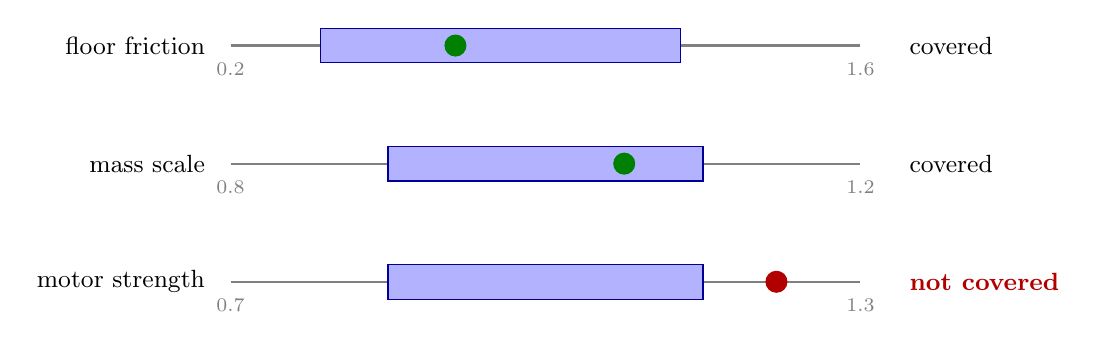
\begin{tikzpicture}[x=1cm,y=1cm]
  \foreach \nm/\mn/\mx/\lo/\hi/\re/\col [count=\i] in {floor friction/0.2/1.6/0.4/1.2/0.7/green!50!black, mass scale/0.8/1.2/0.9/1.1/1.05/green!50!black, motor strength/0.7/1.3/0.85/1.15/1.22/red!70!black}{
    \pgfmathsetmacro{\xl}{(\lo-\mn)/(\mx-\mn)*8}
    \pgfmathsetmacro{\xh}{(\hi-\mn)/(\mx-\mn)*8}
    \pgfmathsetmacro{\xr}{(\re-\mn)/(\mx-\mn)*8}
    \pgfmathsetmacro{\yy}{-1.5*\i}
    \node[anchor=east,font=\small] at (-0.2,\yy) {\nm};
    \draw[gray,thick] (0,\yy) -- (8,\yy);
    \node[font=\scriptsize,gray,anchor=north] at (0,\yy-0.1) {\mn};
    \node[font=\scriptsize,gray,anchor=north] at (8,\yy-0.1) {\mx};
    \fill[blue!30] (\xl,\yy-0.22) rectangle (\xh,\yy+0.22);
    \draw[blue!60!black] (\xl,\yy-0.22) rectangle (\xh,\yy+0.22);
    \fill[\col] (\xr,\yy) circle (0.14);
  }
  \node[anchor=west,font=\small] at (8.5,-1.5) {covered};
  \node[anchor=west,font=\small] at (8.5,-3.0) {covered};
  \node[anchor=west,font=\small,red!70!black] at (8.5,-4.5) {\textbf{not covered}};
\end{tikzpicture}
\captionof{figure}{Randomised ranges (blue bars) in the simulator and the true value on the real robot (dots). The real motors are stronger than anything the policy saw during training (red), so the transfer is likely to fail until the range is widened.}\label{fig:rl6_ranges}
\end{center}

Typical quantities that are randomised: floor friction, the mass of every body part, the position of the centre of mass, motor strength and PD gains, sensor noise, latency, and random pushes during walking. The code for one sample is simple:

\begin{verbatim}
import random

def sample_world():
    return {
        "friction":       random.uniform(0.4, 1.2),
        "mass_scale":     random.uniform(0.9, 1.1),
        "motor_strength": random.uniform(0.85, 1.15),
        "latency_steps":  random.choice([0, 1, 2]),
        "push_force_N":   random.uniform(0.0, 50.0),
    }
\end{verbatim}

\begin{keyidea}[The width of the ranges]
Too narrow: the real world is outside, and the policy fails. Too wide: the policy has to be careful about everything and becomes slow and conservative. Use measurements of the real robot to choose ranges that are as narrow as possible but still contain the truth.
\end{keyidea}

\section*{Latency}
A real signal needs time. If the sensors, the computer and the motor together need $40$\,ms, the action chosen now reaches the motor $40$\,ms later. At $50$ Hz one step is $20$\,ms, so $40$\,ms is $2$ steps. The policy then acts on a situation that is already two steps old, and acts on it two steps too late.

\begin{center}
\begin{tikzpicture}
  \draw[-{Stealth},thick] (0,0) -- (11,0) node[right,font=\small]{time};
  \foreach \x/\l in {0/0,2/20,4/40,6/60,8/80,10/100}{
    \draw (\x,0.1) -- (\x,-0.1) node[below,font=\scriptsize]{\l\,ms};
  }
  \node[draw,rounded corners,fill=blue!10,font=\scriptsize,minimum height=0.7cm] at (1,1.0) {sensor reading};
  \node[draw,rounded corners,fill=orange!15,font=\scriptsize,minimum height=0.7cm] at (3,1.0) {policy};
  \draw[-{Stealth},thick,red!70!black] (0,2.0) -- node[above,font=\scriptsize]{delay $40$ ms $=2$ steps} (4,2.0);
  \node[draw,rounded corners,fill=green!10,font=\scriptsize,minimum height=0.7cm] at (5,1.0) {motor moves};
\end{tikzpicture}
\captionof{figure}{Latency: between the measurement (at $0$ ms) and the movement of the motor (from $40$ ms on) the robot already moved on.}\label{fig:rl6_latency}
\end{center}

Two remedies are common: randomise the latency during training (as in the code above), and give the policy the \emph{previous action} as part of its observation so that it can account for movements that are still on their way.

\section*{Measure the real robot: system identification}
Instead of guessing the simulator parameters we can measure them: weigh the robot parts, let a joint follow a test motion and compare the real angle curve with the simulated one. The simulator is then adjusted until the curves agree. A simple measure of the difference is the \textbf{root mean square error}
\[
\text{RMS}=\sqrt{\frac1n\sum_{i=1}^{n}\bigl(q_i^{\text{real}}-q_i^{\text{sim}}\bigr)^2}.
\]

\begin{example}
Four angle differences between the real and the simulated joint are $0.02$, $-0.03$, $0.01$ and $0.04$\,rad. The squares are $0.0004,\,0.0009,\,0.0001,\,0.0016$ with the mean $0.00075$, so $\text{RMS}=\sqrt{0.00075}\approx0.027$\,rad (about $1.6^\circ$).
\end{example}

\section*{Only use what the real robot can measure}
In a simulator everything is known exactly: the true body speed, the true position of the ball, the friction coefficient. The real robot does not have these numbers. If the policy uses such ``privileged'' information during training it will have nothing to work with on the real robot. The observation of the policy should contain only quantities that the real robot can measure or estimate: joint angles and speeds from the encoders, orientation and rotation rate from the IMU, the last action, and the command. Estimating quantities that cannot be measured directly (position on the field, ball position) is the topic of the part on state estimation and perception.

\section*{From the simulator to the field}
Moving a policy to a real humanoid is done in small, safe steps (Figure~\ref{fig:rl6_pipeline}). Each step can send the policy back to the beginning.

\begin{center}
\begin{tikzpicture}[node distance=0.35cm, box/.style={draw,rounded corners,thick,minimum width=2.1cm,minimum height=1.5cm,align=center,font=\scriptsize,text width=2.0cm}]
  \node[box,fill=blue!10] (a) {1. Train with randomisation};
  \node[box,fill=blue!10,right=of a] (b) {2. Test in a second simulator};
  \node[box,fill=orange!15,right=of b] (c) {3. Robot hanging in the air};
  \node[box,fill=orange!15,right=of c] (d) {4. Standing on the floor, slow};
  \node[box,fill=green!10,right=of d] (e) {5. Full test on the field};
  \foreach \x/\y in {a/b,b/c,c/d,d/e}{\draw[-{Stealth},thick] (\x) -- (\y);}
\end{tikzpicture}
\captionof{figure}{A safe path from the simulator to the real robot. If a step fails, go back and improve the training.}\label{fig:rl6_pipeline}
\end{center}

\begin{stepbox}{Safety checklist for the first test of a new policy}
\begin{enumerate}[nosep]
  \item Check the battery and the cables. Clear the area around the robot.
  \item Make sure that an emergency stop is within reach, and that a person is ready to catch the robot.
  \item First test with the robot hanging in a safe holder: do the joints move smoothly?
  \item Start with low gains and slow commands, then increase them step by step.
  \item Record all sensor data and actions (a log), so that you can compare reality with the simulation afterwards.
\end{enumerate}
\end{stepbox}

\begin{aibox}
The same pipeline, train in simulation $\to$ randomise $\to$ test carefully $\to$ deploy, is how learned walking, getting up and kicking motions arrive on humanoid robots. Part~IX of this book follows this path with a specific robot, from setting up a simulator to the first steps on the real floor.
\end{aibox}

\section*{Practice problems}
\begin{enumerate}[label=\textbf{\thechapter.\arabic*}]
  \item A simulator produces $100\,000$ steps per second in total and the policy runs at $50$ Hz. How many seconds of robot experience are collected per second of computer time? How many hours of robot time are collected in $10$ minutes?
  \item A PD controller with $K_p=40$ and $K_d=1$ controls a joint with target $0.5$\,rad, angle $0.3$\,rad and speed $1$\,rad/s. Compute $\tau$. What is $\tau$ if the joint is at the target ($q=0.5$) and still moves with $\dot q=2$\,rad/s? What does that mean physically?
  \item The delay between a measurement and the motor reaction is $30$\,ms. How many control steps is that at $100$ Hz? At $50$ Hz (round up)?
  \item Friction is randomised uniformly between $0.4$ and $1.2$. (a) Is the real value $0.7$ covered? (b) And the value $1.4$? (c) How likely is a sample between $0.6$ and $0.8$?
  \item A robot has the nominal mass $20$\,kg and the mass is randomised by $\pm10\,\%$. Give the range in kg and the mass for the scale factors $0.95$ and $1.08$.
  \item Compute the RMS error for the differences $0.05,\,-0.02,\,0.03,\,0.00,\,-0.04$\,rad.
  \item Which of these quantities may the policy use as an input on the real robot? (a) joint angle from an encoder, (b) the true friction coefficient, (c) orientation from the IMU, (d) the exact position of the ball in world coordinates as given by the simulator, (e) the previous action.
  \item Explain what can go wrong if the randomisation ranges are far too wide.
  \item[\textbf{\thechapter.9}] \texttt{[code]} Use the function \texttt{sample\_world()} to draw $1000$ worlds and compute the average friction and the share of worlds with latency $2$. Compare with the expected values.
  \item[\textbf{\thechapter.10}$\star$] Why does it help the policy to receive its previous action as an input when there is latency? Think about what it cannot know otherwise.
\end{enumerate}
